% \begin{figure}
%     \centering
%     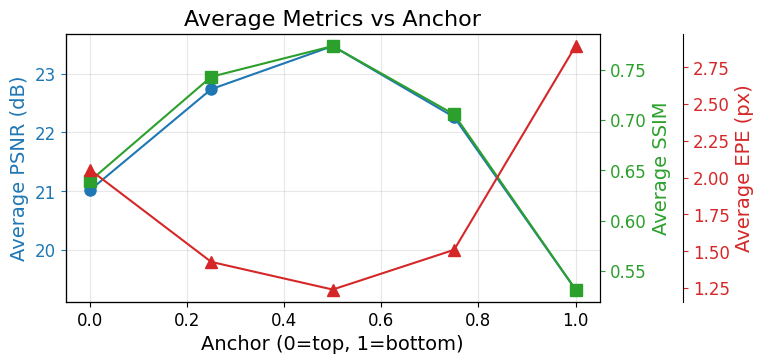
\includegraphics[width=\linewidth]{Figures/rs-diff.png}%
%     \vspace{-2mm}
%     \caption{Demonstration of the proposed \textit{anchor point} formulation using a representative rolling shutter depth framework~\cite{RS-Diffusion}. Our theory predicts an optimal anchor point at $N/2$. By modifying only the anchor-point selection, while keeping the original implementation and pretrained weights unchanged, we observe substantial performance improvements \textit{without retraining}. The plotted results confirm that performance peaks near the theoretically predicted anchor location. \JI{What is N? - revise and address}
%     %As a demonstration of our \textit{anchor point} idea, consider the state-of-the-art paper RS Diffusion \cite{RS-Diffusion}. Our theory predicts an anchor point of $\frac{N}{2}$, which the authors of \cite{RS-Diffusion} do not use -- instead, they use an anchor point of $0$ (most prior RS researchers use an arbitrary anchor point by default). By using \textit{their code} and \textit{their dataset}, and by changing only a \textit{single line of code} to vary the anchor point, we can achieve significantly better results \textit{with no retraining}. The graphs show the optimal value is at our predicted anchor point $\frac{N}{2}$.
%     } 
%     \label{fig:rs-diff_comp}
%     \vspace{-5mm}
% \end{figure}


\section{Introduction}

Rolling shutter (RS) effects arise from row-by-row image readout, causing each scanline to be captured at a different time rather than simultaneously as in global shutter (GS) imaging. In dynamic scenes, this temporal offset induces complex geometric distortions that depend on both camera ego-motion and scene dynamics. RS cameras remain ubiquitous in modern robotic systems because they are compact, power-efficient, and cost-effective compared to global shutter alternatives\cite{4549748}. 
% While prior work on rolling shutter correction (RSC) has shown progress for mild or structured distortions, performance often degrades under large, nonlinear RS effects frequently encountered in real robotic deployments\ref{fig:collocated_results}. As a result, reliable monocular depth estimation from single-view RS imagery remains challenging. 

Prior work addresses RS correction using geometric and learning-based methods. Rolling-shutter-aware pose estimation has also been explored in robotics to mitigate downstream effects.
Despite these advances, existing methods struggle with single-frame images under large distortions, often assuming mild motion, requiring extra sensors, or relying on temporal context. Moreover, learning-based methods fix a temporal reference implicitly, yet the impact of this choice on geometric consistency and depth prediction remains underexplored. Due to this lack of exploration, reliable monocular depth estimation from large RS distortions remains a challenge.

% \JI{It is great that the first paragraph mentions "what is the problem and why is this important". Although needs citations. The second paragraph is missing where you talk about "what other people have done and what specific challenges remain". The second paragraph is missing}


% "what are you proposing"
% A central component of our approach is the \textbf{anchor point}, a temporal reference that specifies which GS frame an RS image corresponds to. \textit{While the idea is simple, many modern RSC algorithms don't optimize their selection of anchor point \cite{RS-Diffusion}, \cite{DeepUnrollNet}}. This change alone yields a significant performance improvement without retraining (Fig.~\ref{fig:teaser_results}). Through this and additional analysis, we show that anchor point selection strongly influences correction quality and downstream depth estimation, particularly under severe RS distortions. We analyze anchor point configurations systematically and identify selections that yield stable and geometrically consistent reconstructions.
% %\JI{I dont think you motivated your method well. Will talk more in person}

% % "how we evaluate it"
% To evaluate these effects in realistic settings, we introduce a new co-located RS-GS \textbf{dataset} designed to capture the motion profiles and imaging artifacts common in robotic systems. Using a custom beam-splitter camera rig with explicit delay control, we precisely specify anchor points during data capture, enabling fine-grained analysis of RS correction performance under large distortions. We evaluate our approach using a two-stage visual foundation pipeline that performs RSC followed by monocular depth estimation. Across synthetic and real-world benchmarks, our results demonstrate improved robustness to extreme RS distortions and large ego-motion.

%Attempt to get back real estate by fusing past two parag.
A central component of our approach is the \textbf{anchor point}, a temporal reference that specifies which GS frame a RS image is aligned to.  \draft{Existing RS correction methods implicitly select a temporal reference frame, yet the consequences of this choice have not been systematically analyzed \cite{RS-Diffusion,DeepUnrollNet}. We formalize this reference as an anchor point, derive conditions governing its optimal selection, and demonstrate experimentally that anchor-point choice is a first-order factor affecting both rolling shutter correction and downstream monocular depth estimation.} Adjusting this reference alone can yield substantial performance gains without retraining (see Fig.~\ref{fig:teaser_results}). For comprehensive evaluation, we introduce a new collocated RS–GS dataset captured with a beam-splitter rig that provides explicit control over anchor points. Using this dataset and a two-stage visual foundation pipeline for RS correction and depth estimation, we demonstrate improved robustness to large distortions and aggressive ego-motion across synthetic and real-world benchmarks.
% While conceptually simple, many modern RSC methods fix this reference implicitly and do not optimize its selection
\vspace{1mm}
\noindent
{Our contributions are as follows:}
\begin{enumerate}
    \item We introduce the concept of ``\textit{anchor point}" as a temporal reference for rolling shutter to global shutter (RS-GS) alignment, and provide a systematic analysis of its role in rolling shutter correction and monocular depth estimation under severe geometric distortions (Sect. III).

    %\item We introduce the concept of \textbf{anchor point}, a temporal reference for RS-GS alignment, and analyze its impact on rolling shutter correction and monocular depth estimation under large distortions (\figurename~ {3}).
    \item We present a new collocated RS-GS dataset with explicit anchor-point control, designed to capture realistic robotic motion with large ego-motion effects and practical imaging artifacts (Figs.~3-5).

    %We present a new co-located RS-GS dataset with explicit anchor-point control, designed to reflect realistic robotic motion and imaging artifacts (\figurename~{3, 4, 5}).
    \item We conduct extensive ablation studies across both synthetic and real-world data to quantify the influence of anchor point selection on reconstruction accuracy and depth consistency (Figs.~6-7, Tables~II-III).

    %We provide extensive ablation studies evaluating anchor point selection across synthetic and real data (\figurename~ {6, 7}, Table 2-3).
    \item We develop a two-stage foundation-model-based pipeline and demonstrate its effectiveness for rolling shutter correction and monocular depth estimation under extreme distortions and aggressive ego-motion (\figurename~8, Table~I).
    %We demonstrate the effectiveness of our approach for RS correction and monocular depth estimation under extreme distortions and large ego-motion with a two-stage foundation model pipeline (\figurename~{8}, Table~{1}).
    \item We validate the proposed system at 400\,ms end-to-end latency on a legged robot with a collocated sensor setup (\figurename~10).
    % , including live 3D reconstruction visualization
    %We demonstrate our system in near-real time (400ms latency) with a co-located system on top of a robot with reconstruction visualization (\figurename~ {10}).
\end{enumerate}

The proposed framework demonstrates promise for near-real-time RSC by mobile robots under challenging motion conditions. Its validation on a legged robot, subjected to rapid, irregular ego-motion, highlights its viability in real-world applications.

